\newpage
\section{Chain Rule}
March 27, 2023
\begin{itemize}
	\item For gradient functions:
		\begin{align*}
		f\left( \vec{x}+\vec{h}  \right) - f\left( \vec{x}\right) = \vec{y} \cdot  \vec{h} + o\left( \vec{h} \right) \\
		\implies \vec{y} = \nabla f = \text{gradient of} f\\
		\text{which is } \left( f_x, f_y, f_z \right) 
	\end{align*}
\item directional derivative, allow us to take the derivative with any direction we choose:
	\begin{equation}
		f_{\hat{u}} = \nabla f \cdot  \hat{u}
	\end{equation}
	\begin{example}
		We have $z = f\left( x,y \right) = A + x + 2y - x^2 - 3y^2$, an eliptical parabolic hill. With the starting point of $\left( 0,0,A \right) $, our job is to get down the hill, following the path of steepest descent. We will calculate a few things, and put together the process. We have partial derivatives:
		\begin{align*}
			f_x &= 1-2x \\
			f_y &= 2-6y \\
		.\end{align*}
		And we have:
		\begin{equation}
			\nabla f = \left( 1-2x \right) \hat{i} + \left( 2-6y \right) \hat{j}
		\end{equation}
		This is the gradient, pointing UPHILL, to get the down hill:
		\begin{equation}
			-\nabla f = \left( 2x-1 \right) \hat{i} + \left( 6y-2 \right) \hat{j}
		\end{equation}
		We have the path of steepest descent, we call it curve $C: r\left( t \right)  = x\left( t \right) \hat{i} + y\left( t \right) \hat{j}$, Note: This path will have direction same as the steepest descent path.
		\begin{align*}
			x'\left( t \right)  &= 2x\left( t \right) -1\\
			y'\left( t \right)  &= 6y\left( t \right)  - 2\\
			\therefore \frac{dy}{dx} &=  \frac{6y-2}{2x-1} \\
		.\end{align*}
		This is a separable equation, we can solve it to find the actual path from the directions. After separating we can integrate directly.
		\begin{align*}
			\frac{dy}{6y-2}&= \frac{dx}{2x-1} \\
			\implies \frac{1}{6} \ln|6y-2| &=  \frac{1}{2}\ln|2x-1| + C \\
			\therefore 6y-2 &= \left( 2x-1 \right) ^3e^C \\
		.\end{align*}
		We need to find what the integration constant: $e^C$ is, so we start from our initial condition: $x=0, y=0$
		\begin{align*}
			-2 &= \left( -1 \right) ^3e^C \\
			\therefore e^c &= 2 \\
			\therefore 3y = \left( 2x-1 \right) ^3+1
		.\end{align*}
		And this is our steepest descent path. Everywhere along the curve $C$, the direction is the steepest downhill descent, and the path itself is the steepest descent
	\end{example}
\item The Chain Rule:
	\begin{theorem}
		Chain Rule Along a Curve:
		\begin{align*}
			\frac{d}{dt}\left[ f\left(\vec{r}\left( t \right)  \right)  \right] &= \nabla f\left( \vec{r}\left( t \right)  \right) \cdot \vec{r}~'\left( t \right) \\
			&= \frac{\partial f}{\partial x} \cdot \frac{d x}{d t} +\frac{\partial f}{\partial y} \cdot \frac{d y}{d t} +\frac{\partial f}{\partial z} \cdot \frac{d z}{d t}  \\
			&= \nabla f \cdot  \vec{T} \cdot \left( \frac{ds}{dt} \right)  \\
		\end{align*}
		which is unit tangent $\times $ change in length
	\end{theorem}
	\begin{example}
		Assume we have function $\vec{r}\left( t \right)  = x\left( t \right) \hat{i} + y\left( t \right) \hat{j}$ which describes path or position, say:
		\begin{equation}
			\vec{r}\left( t \right)  = \left( t^3, \cos t \right) 
		\end{equation}
		and we have a Temeprature function that's dependent on position
		\begin{equation}
			T\left( x,y \right)  = xy^2
		\end{equation}
		What is the change in temperature as I go along the path $\vec{r}$ We have:
		\begin{align*}
			\nabla T &= \left( y^2 , 2xy\right) \\
			\vec{r}~' &= \left( 3t^2, -\sin t \right)  \\
		.\end{align*}
		Solving for chain rule:
		\begin{align*}
			\therefore \frac{dT}{dt}&= \nabla T \cdot  \vec{r}~' \\
			&= y^2\cdot 3t^2-2xy\sin t \\
			&= 3t^2\cos^2 t - 2t^3\cos t \sin t \\
		.\end{align*}
		Or we can solve using the old fashioned method, by subbing $x,y$ from $\vec{r}$
		\begin{equation}
			T = xy^2 = t^3 \cos^2 t
		\end{equation}
		\begin{equation}
			\therefore \frac{dT}{dt} = 3t^2\cos^2t - 2t^3\cos t \sin t \\
		\end{equation}
	\end{example}
	\begin{example}
		We have a room, $V = \ell\cdot h\cdot d $. Say:
		\begin{align*}
			\ell \text{ is increasing at:} \frac{d\ell}{dt} &=  3 \frac{\text{m}}{\text{s}} \\
			h \text{ dec } \frac{dh}{dt}&= -2 \frac{\text{m}}{\text{s}} \\
			d \text{ inc } \frac{dd}{dt} &= 5 \frac{\text{m}}{\text{s}} \\
		.\end{align*}
		starting from $ \ell = 2, h = 3, d = 4$, and we create a $q$ vector that is the vector containing these 3 components.
		\begin{equation}
			V\left( t \right) = \ell\left( t \right)  \cdot  h\left( t  \right) \cdot d\left( t \right) \text{ and } \vec{q}\left( t \right) = \left( \ell, h, d \right)  \\
		\end{equation}
		Using chain rule for multivariable functions:
		\begin{align*}
			\frac{dV\left( t \right) }{dt}&= \nabla V\left( \vec{q}\left( t \right)  \right) \cdot  \vec{q}~'\left( t \right)\\
										  &\implies \nabla V = \left( \frac{\partial V}{\partial \ell} , \frac{\partial V}{\partial h} , \frac{\partial V}{\partial d}  \right)  = \left(hd, \ell d , h \ell \right) \\
										  &\implies \vec{q}~'\left( t \right) = \left(\frac{d\ell}{dt}, \frac{dh}{dt}, \frac{dd}{dt} \right)  = \left( 3, -2, 5 \right)  
		\end{align*}
		Therefore, at the initial point of $\left( 3,-2,5 \right) $
		\begin{equation}
			\frac{dV}{dt} = 3hd - 2\ell d + 5 \ell h = 3 \cdot 3\cdot 4 - 2\cdot 2\cdot 4 +5\cdot 2\cdot 3 = 50 \frac{\text{m}^3}{\text{s}}		
		\end{equation}
		As a comparison, we can also solve this using the traditional method of subbing in variables:
		\begin{align*}
			\ell &=  2+3t \\
			h &= 3-2t \\
			d &=  4+5t \\
		\end{align*}
		We can also solve using the old fashioned method:
		\begin{equation}
			\therefore  V = \left( 2+3t \right) \left( 3-2t \right) \left( 4+5t \right)  \\
		\end{equation}
	\end{example}
	\begin{idea}
		We can have x,y given as functions with two parameters, this will represent a SURFACE in 3D, not a curve anymore.
		\begin{align*}
			x &= x\left( t,s \right) \\
			y &=  y\left( t,s \right)  \\
			f &= f\left( x,y \right)  \\
		.\end{align*}
		But we can still follow the same process of applying chain rule, we just have two rates of changes now
		\begin{align*}
			\frac{\partial f}{\partial t}  &=  \frac{\partial f}{\partial x} \frac{\partial x}{\partial t}  + \frac{\partial f}{\partial y}  \frac{\partial y}{\partial t}  \\
			\frac{\partial f}{\partial s} &= \frac{\partial f}{\partial x} \frac{\partial x}{\partial s} + \frac{\partial f}{\partial y}  \frac{\partial y}{\partial s}  \\
		.\end{align*}
	\end{idea}
\item \textbf{Implicit Differentiation:}\\
	Let us have this function
	\[
	u\left( x,y \right) = 0 \implies \frac{dy}{dx} = ?
	.\] 
	Let $x = t$, $y = y\left( t \right) $, Then we have $u = u\left( t,y\left( t \right)  \right) $ because we chose $x=t$, so $y$ must be a function of $t$
	\begin{align*}
		\frac{du}{dt} &= \frac{\partial u}{\partial x} \frac{d x}{d t} + \frac{\partial u}{\partial y} \frac{d y}{d t}  \\
	\end{align*}
	Following the original statement that $u\left( x,y \right) =0$, $u\left( t, u\left( t \right)   \right) = 0$, $\therefore \frac{du}{dt} = 0$ since $u$ is constant.
	\[
	x = t\\
	\therefore \frac{dx}{dt}= 1 \text{ and } \frac{dy}{dt} = \frac{dy}{dx}
	.\] 
	Therefore
	\begin{align*}
		0 &= \frac{\partial u}{\partial x}  + \frac{\partial u}{\partial y} \frac{\partial y}{\partial x} \\
		\implies \frac{dy}{dx} &=  -\frac{\frac{\partial u}{\partial x} }{\frac{\partial u}{\partial y} } \\
	\end{align*}
	\begin{example}
		We have:
		\begin{equation}
			x^4 + 4x^3 y + y^4 = 1 \implies u = x^4 + 4x^3y + y^4 - 1 = 0
		\end{equation}
		Rearranged into $u$, now we just solve for derivative of $u$ with respect to each variables
		\begin{align*}
			\frac{du}{dx} &=  4x^3 + 12x^2 y \\
			\frac{du}{dy} &=  4x^3 + 4y^3 \\
		.\end{align*}
		Partial derivatives are easy to find, and we just have to find the ratio
		\begin{equation}
			\therefore  \frac{dy}{dx} = - \frac{4x^3 + 12x^2y}{4x^3 + 4y^3} = - \frac{x^2\left( x+3y \right) }{x^3+y^3}
		\end{equation}
	\end{example}
\item \textbf{14.4 and 14.6: Tangent Plane and Linear Approximation}\\
	\begin{definition}
		Level curve is the curve on a plane where the "height" doesn't change.
	\end{definition}
	\begin{example}
		
	Returning to the parabolic hill example: \\
	Say we have $z\left( x,y \right)  = 20 - x^2 - y^2$, we start from $P\left( 1,2 \right) $. The level curve at this point, that retains the "height" value of '15' will be:
	\[
	 C = 20-x^2 - y^2, P\left( 1,2 \right) \\
	 \therefore  C = 20-1^2-2^2 = 15
	.\] 
	$C = 15 \implies 20 - x^2 - y^2 = 15 \implies$ level curve: $x^2 + y^2 =5$ \\
	We have the tangent vector $\vec{t}$. (not the unit tangent, but also perpendicular to $\vec{r}$):
	\begin{align*}
	\text{Starting point: }	\vec{r}\left( 1,2 \right)  \\
		\therefore  \vec{t} \cdot  \vec{r} = \left( t_1,t_2 \right) \cdot  \left(1,2  \right)  =  0 \\
		\implies t_1\cdot 1+t_2 \cdot 2 = 0
	\end{align*}
	Choose $t_1 = 2, t_2 = -1$ $\therefore \vec{t} = \left( 2,-1 \right) $ is the tangent vector
	\begin{align*}
		\nabla z \cdot  \vec{t} &=  \left( -2x, -2y \right)  \cdot  \left( 2,-1 \right)  \\
	&= -4x + 2y \\
	\text{at }\left( 1,2 \right)  &=  -4+4 = 0 \\
	\end{align*}
\end{example}
\begin{theorem}
	For level curve, the gradient will be perpendicular to the tangent at a specific point. \\
	Proof: let's define a function $f$ to represent the curve:
	 \begin{align*}
		 f\left( x,y \right)  &= C, \text{ let }\vec{r}\left( t \right)  = x\left( t \right) \hat{i} + y\left( t \right) \hat{j} && \vec{t} = \vec{r}~'\left( t \right) \\
		\implies f\left( \vec{r}\left( t \right)  \right)  &=  C \\
	.\end{align*}
	\begin{align*}
		\frac{d}{dt}f\left( \vec{r}\left( t \right)  \right)  &=  \nabla f\left( \vec{r} \right)  \cdot  \vec{r}~' \\
															  &= \frac{dC}{dt} && [\text{level curve: $C$ is constant}]\\
		&= 0 \\
	.\end{align*}
	along the level curve, the tangent vector dot the gradient is 0, so we can conclude that gradient is NORMAL to the normal curve:
	\[
	\nabla f \cdot  \vec{r}~' = 0 \text{ or } \nabla f\left( \vec{r} \right) \text{ is perpendicular to } \vec{r}~'
	.\] 
	Since gradient function is perpendicular to tangent, we can define tangent to be:
	\[
	\nabla f \cdot  \vec{r} = \nabla f \cdot  \vec{t} = 0
	.\] 
	\begin{equation}
		\vec{t} = \left( \frac{\partial f}{\partial y} , - \frac{\partial f}{\partial x}  \right) 
	\end{equation}
	This way we always satisify the "perpendicular" property between gradient and tangent.
	\begin{align*}
		\implies \nabla f \cdot  \vec{t} &= \left( \frac{\partial f}{\partial x} , \frac{\partial f}{\partial y}  \right) \cdot  \left( \frac{\partial f}{\partial y}, -\frac{\partial f}{\partial x}   \right)   \\ 
		&= \frac{\partial f}{\partial x} \frac{\partial f}{\partial y} - \frac{\partial f}{\partial x} \frac{\partial f}{\partial y}  \\
		&= 0 \\
	\end{align*}
	\end{theorem}
	\begin{figure}[htpb]
		\centering
		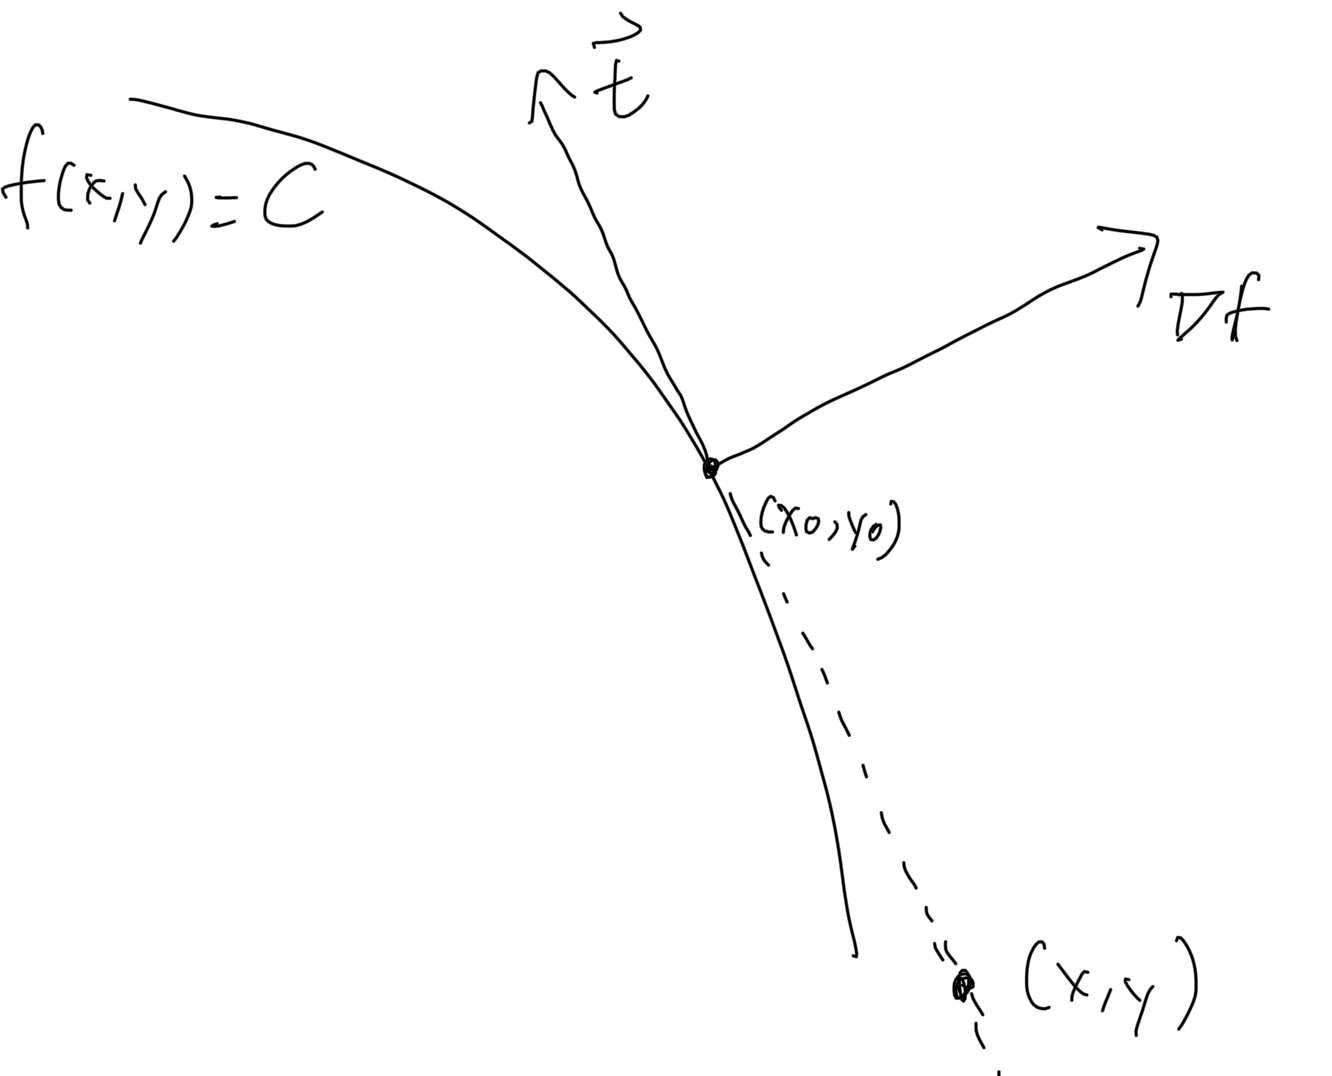
\includegraphics[width=0.3\textwidth]{"./figures/normal_tangent_line.jpg"}
		\caption{normal and tangent lines}
		\label{fig:}
	\end{figure}
\item Refer to the above figure, we can see that for every level curve $C$ at every point, there will be a gradient $\nabla f$ and a tangent $\vec{t}$. Most importantly, they are orthagonal to each other:
	\begin{equation}
		\nabla f \cdot  \vec{t} = 0
	\end{equation}
	Using this, we can draw normal and parallel lines to the curve.
	\begin{theorem}
		To draw parallel line to point $\left( x_0,y_0 \right) $, we want to describe any point that lies on the line of $\vec{t}$. The vector $\left( x_0,y_0 \right) \to \left( x,y \right) =\left( x-x_0,y-y_0 \right) $ and is orthagonal to $\nabla f$:
		\begin{align*}
			\left( x-x_0,y-y_0 \right) \cdot \nabla f &=  0 \\
			\left( x-x_0,y-y_0 \right) \cdot \left( \frac{\partial f}{\partial x} , \frac{\partial f}{\partial y}  \right) &= 0 \\
			\therefore \left( x-x_0 \right) \cdot \frac{\partial f }{\partial x} \left( x_0,y_0 \right) +\left( y-y_0 \right) \cdot \frac{\partial f}{\partial y} \left( x_0,y_0 \right) &= 0 \\
		\end{align*}
		To draw normal line, we apply the same procedure, but now $\left( x,y \right) $ lies on $\nabla f$ and is orthagonal to $\vec{t}$:
		\begin{align*}
			\left( x-x_0,y-y_0 \right) \cdot \vec{t} &=  0 \\
			\left( x-x_0,y-y_0 \right) \cdot \left( \frac{\partial f}{\partial y} , -\frac{\partial f}{\partial x}  \right) &= 0 \\
			\therefore \left( x-x_0 \right) \cdot \frac{\partial f }{\partial y} \left( x_0,y_0 \right) -\left( y-y_0 \right) \cdot \frac{\partial f}{\partial x} \left( x_0,y_0 \right) &= 0 \\
		\end{align*}
	\end{theorem}

\end{itemize}
